\documentclass{article}

\title{Optimization}
\author{Vladimir Feinberg}

\usepackage{nicefrac}
\usepackage[hidelinks]{hyperref}
\usepackage{xcolor}
\usepackage{url}
\usepackage{lmodern}
\usepackage{amsmath}
\usepackage{amsthm}
\usepackage{amssymb}
\usepackage{amsfonts}
\usepackage{enumerate}
\usepackage{graphicx}
\usepackage{fullpage}
\usepackage{bbm}
\usepackage{caption}
\usepackage{mathrsfs}
\usepackage[all]{xy}

\newcommand{\pa}[1]{ \left({#1}\right) }

\def \N {\mathbb{N}}
\def \Nbr {\mathcal{N}}
\def \Q {\mathbb{Q}}
\def \F {\mathbb{F}}
\def \then {\implies &}
\def \oif {\Longleftrightarrow &\,}
\def \given {\text{Given }&}
\def \assume {\text{Assume }&}
\def \thfr {\therefore &\enskip}
\def \bij {\leftrightarrow}
\def \inj {\rightarrowtail}
\def \sur {\twoheadedrightarrow}
\def \Z {\mathbb{Z}}
\def \R {\mathbb{R}}
\def \C {\mathbb{C}}
\def \T {\mathbb{T}}
\def \iff {\Longleftrightarrow}
\def \kron {\boldsymbol\delta}
\def \indicator {\mathbbm{1}}

\def\Ta{\textbf{a}}
\def\Tm{\textbf{m}}
\def\Tb{\textbf{b}}
\def\Tc{\textbf{c}}
\def\Td{\textbf{d}}
\def\Te{\textbf{e}}
\def\Tv{\textbf{v}}
\def\Tx{\textbf{x}}
\def\Tw{\textbf{w}}
\def\Ty{\textbf{y}}
\def\Tk{\textbf{k}}
\def\Tt{\textbf{t}}
\def\Tz{\textbf{z}}
\def\Tl{\textbf{l}}
\def\quotient{\mathclose{}/\mathopen{}}
\def\Tf{\textbf{f}}
\def\Th{\textbf{h}}
\def\Tg{\textbf{g}}
\def\sumn{\sum_{n=0}^\infty}
\def\limn{\lim_{n\rightarrow\infty}}
\def\prodn{\prod_{n=0}^\infty}

\def\bsz{\textbf{0}}
\def\bs1{\textbf{1}}
\def\bsa{{\boldsymbol\alpha}}
\def\bse{{\boldsymbol\eta}}
\def \bss{ {\boldsymbol\sigma}}
\def \bsth{ {\boldsymbol\theta}}

\DeclareMathOperator{\conv}{conv}
\DeclareMathOperator\cat{cat}
\DeclareMathOperator\adj{adj}
\DeclareMathOperator{\Laplace}{Laplace}
\DeclareMathOperator\Poisson{Poisson}
\DeclareMathOperator\Id{Id}
\DeclareMathOperator\Uniform{Uniform}
\DeclareMathOperator\mathProb{\mathbb{P}}
\def\P{\mathProb} % need to overwrite stupid paragraph symbol
\DeclareMathOperator\mathExp{\mathbb{E}}
\def \E {\mathExp}


\newcommand{\stc}[1]{\widetilde{#1}}   
\newcommand{\set}[2]{ \left\{ #1 \,\middle|\, #2 \right\} }
\newcommand{\idx}[3]{ \left\{ #1 \right\}_{ #2 }^{ #3 } }
\newcommand{\card}[1]{\left\vert{#1}\right\vert}
\newcommand{\colv}[1]{\begin{pmatrix} #1 \end{pmatrix}}
\newcommand{\mat}[1]{\begin{pmatrix} #1 \end{pmatrix}}
\newcommand{\detmat}[1]{\begin{vmatrix} #1 \end{vmatrix}}
\newcommand{\spanb}[1]{\text{span}\{ #1 \}}
\newcommand{\abs}[1]{\left|#1\right|}
\newcommand{\opcat}[1]{#1^{\text{op}}}
\newcommand{\Inner}[1]{\left\langle #1 \right\rangle}
\newcommand{\Innercpy}[1]{\Inner{ #1, #1 }}
\newcommand{\norm}[1]{\left\| #1 \right\|}% use instead of $\|x\|$

\def\eqd{\mathrel{\overset{\Delta}{=}}}

\DeclareMathOperator{\diag}{diag}
\DeclareMathOperator{\vcdim}{VC-dim}
\DeclareMathOperator*{\Err}{\text{err}}
\DeclareMathOperator*{\ErrE}{\mathbb{E}}
\DeclareMathOperator{\Tr}{tr}
\DeclareMathOperator{\Dim}{dim}
\DeclareMathOperator{\Rank}{rank}
\DeclareMathOperator*{\argmin}{argmin}
\DeclareMathOperator*{\proj}{proj}
\DeclareMathOperator{\Ker}{ker}
\DeclareMathOperator{\Diam}{diam}
\DeclareMathOperator{\Int}{int}
\DeclareMathOperator{\Clo}{clo}
\DeclareMathOperator{\sgn}{sgn}
\DeclareMathOperator{\MyRe}{Re}
\DeclareMathOperator{\MyIm}{Im}
\DeclareMathOperator{\image}{image}
\DeclareMathOperator{\colim}{colim}
\DeclareMathOperator{\Supp}{supp}
\DeclareMathOperator{\Var}{var}
\DeclareMathOperator{\Hom}{hom}
\DeclareMathOperator{\Ob}{ob}
\DeclareMathOperator{\El}{el}
\DeclareMathOperator\power{{\mathcal{P}}}
\DeclareMathOperator{\Nat}{Nat}
\DeclareMathOperator{\cone}{cone}
\DeclareMathOperator{\vectorize}{vec}
\DeclareMathOperator{\matricize}{mat}

% probability stuff
\def \sa {{$\sigma$-algebra}}
\def\OR{{\overline{\R}}}
\def\OX{{\overline{X}}}

\def\mcU{{\mathcal{U}}}
\def \mcX {\mathcal{X}}
\def \mcS {\mathcal{S}}
\def \mcY {\mathcal{Y}}
\def \mcH {\mathcal{H}}
\def \mcD {\mathcal{D}}
\def \mcC {\mathcal{C}}
\def \mcA {\mathcal{A}}
\def \mcK {\mathcal{K}}
\def \mcM {\mathcal{M}}
\def\mcG{{\mathcal{G}}}
\def\mcH{{\mathcal{H}}}
\def\mcF{{\mathcal{F}}}
\def\mcB{{\mathcal{B}}}
\def\mcE{{\mathcal{E}}}
\def\mcI{{\mathcal{I}}}
\def\mcQ{{\mathcal{Q}}}
\def\mcM{{\mathcal{M}}}
\def\mcC{{\mathcal{C}}}
\def\mcT{{\mathcal{T}}}
\def\mcO{{\mathcal{O}}}
\def\mcJ{{\mathcal{J}}}

\makeatletter
\DeclareFontFamily{U}  {MnSymbolF}{}
\DeclareSymbolFont{symbolsMN}{U}{MnSymbolF}{m}{n}
\SetSymbolFont{symbolsMN}{bold}{U}{MnSymbolF}{b}{n}
\DeclareFontShape{U}{MnSymbolF}{m}{n}{
    <-6>  MnSymbolF5
   <6-7>  MnSymbolF6
   <7-8>  MnSymbolF7
   <8-9>  MnSymbolF8
   <9-10> MnSymbolF9
  <10-12> MnSymbolF10
  <12->   MnSymbolF12}{}
\DeclareFontShape{U}{MnSymbolF}{b}{n}{
    <-6>  MnSymbolF-Bold5
   <6-7>  MnSymbolF-Bold6
   <7-8>  MnSymbolF-Bold7
   <8-9>  MnSymbolF-Bold8
   <9-10> MnSymbolF-Bold9
  <10-12> MnSymbolF-Bold10
  <12->   MnSymbolF-Bold12}{}
\DeclareMathSymbol{\tbigtimes}{\mathop}{symbolsMN}{2}
\newcommand*{\bigtimes}{%
  \DOTSB
  \tbigtimes
  \slimits@ 
}
\makeatother

% category theory arguments
% more equality: http://tex.stackexchange.com/questions/333629/
\newcommand\superequiv{ \mathrel{\rlap{\raisebox{\fontdimen22\textfont2}{$ = $}}\raisebox{-0.5\fontdimen22\textfont2}{$ = $}}}
\newcommand{\catfst}{{-}}
\newcommand{\catsnd}{{=}}
\newcommand{\cattrd}{{\equiv}}
\newcommand{\catfth}{{\superequiv}}


\newcommand{\nurl}[2]{\href{ #1 }{\color{blue}\underline{#2}}}

\begin{document}

\maketitle

This document contains notes on optimization of DNNs; i.e., the ERM task for a prescribed family of neural networks. Content is mostly from \nurl{http://www.deeplearningbook.org/contents/optimization.html}{Goodfellow's Deep Learning Book}. In the optimization chapter Dr. Goodfellow warns that over the past 30 years of machine learning advances in training speed have mostly been made from making a net that's easier to optimize, not by focusing on the optimization algorithm.

\section{Setting}

To cover a broad NN setting, which, in addition to deep neural networks (DNN) includes recurrent neural networks (RNN), we assume that we wish to minimize empirical risk:
$$
J(\vtheta)=\frac{1}{m}\sum_{i=1}^mL\pa{f\pa{\vx^{(i)}, \vtheta}, y^{(i)}} + \Omega(\vtheta)
$$
Above, $L$ is a fixed, differentiable loss function, as is the regularizer $\Omega$, which is also assumed to be one of several canonical forms. Next, $f$ is a neural network, and therefore a real-valued circuit. Altogether this and backpropagation implies that we have efficient evaluation of $f$ and $\nabla f$ through backprop, as well as some second-order information if desired through Hessian-vector products $\pa{\nabla^2 f}\vv=\nabla\pa{\vv^\top\nabla f}$ (\nurl{http://uhra.herts.ac.uk/handle/2299/4335}{Christianson 1992}).

\section{Stochastic Gradients}

Since $J$ above decomposes easily, we frequently use a stochastic gradient with $B\ll m$ examples,
$$\frac{1}{B}\sum_{i=1}^B\nabla_\vtheta L\pa{f\pa{\vx^{(\sigma_i)}, \vtheta}, y^{(i)}},$$ for random samples $\sigma_i$ uniformly taken from the dataset. Using this for stochastic gradient descent (SGD) as opposed to full gradient descent (GD) enables more efficient derivatives.

\section{Conditioning}

An ill-conditioned Hessian can result in poor optimization. At any given step a twice-differentiable loss will have the following improvement with local Hessian $H$ and gradient $\vg$ assuming step size $\epsilon$:
$$
\epsilon^2 \vg^\top H\vg-\epsilon \vg^\top\vg
$$
Monitoring both of the terms above (which can be done efficiently) during training can help with identifying training issues.

\section{Non-convexity}

$J$ is almost always non-convex in the NN case. This implies that local minima (LM) reached are not necessarily global. However, a global minimum (GM) is not necessary: just a LM close enough to it.

LMs, however, may not always be the root of the problem. Many LMs are induced by symmetry (highly connected nets have combinatorially many symmetries). Recent research shows that LMs concentrate around the GM (\nurl{https://arxiv.org/abs/1412.0233}{Choromanska et al 2014}), so many of these LMs are equivalent to a good solution anyway. Goodfellow claims that most of the time (thanks to early stopping, for instance), most DNN optimizations don't arrive at a critical point of any kind.

A more pertinent problem is that of saddle points (which tend to be much more populous than LMs): locations where the gradient vanishes but the Hessian has both positive and negative eigenvalues (\nurl{https://arxiv.org/abs/1406.2572}{Dauphin et al 2014}). The issue is that along one direction (the linear subspace of positive eigenvectors), the saddle appears to be a LM, and it can take many steps to to get close enough to the bottom of the saddle to locate the direction of negative eigenvalue in the Hessian.

Wide, flat objective regions, ``plateaus,'' are another threat: one that is difficult to circumvent altogether. Momentum is an approach to solve some versions of this problem.

Cliffs may cause a misstep (onto the cliff) to cause a far overshoot, sending the parameters careening very far away (Figure~\ref{fig:pascanu}). This is resolved with gradient clipping.

\begin{figure}[!h]
\centering
{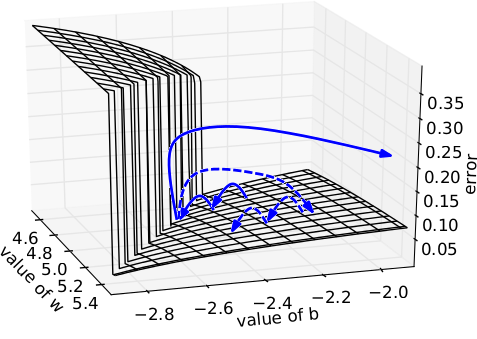
\includegraphics[width=0.5\textwidth]{pascanu2013.png}}
  \caption{Image from Figure 6 of \nurl{https://arxiv.org/abs/1211.5063}{Pascanu et al 2013} demonstrating how cliffs or valleys in optimization landscapes may cause missteps corrected by gradient clipping.}
\label{fig:pascanu}
\end{figure}


\section{Initialization}

Parameters should not be initialized uniformly so as to break symmetry between hidden units; otherwise, the parameters will remain the same during training. This motivates random initialization. Biases, however, are typically constants, heuristically chosen.

Weights are typically Gaussian or uniform, but scale is important. Large scale, which breaks symmetry strongly, must be balanced with stability of the learning algorithm. Heuristics do exist:

\begin{enumerate}
\item ReLU activations, since they're linear, suggest that that the scale of the output for a basic ReLU MLP with $\norm{y}\sim \norm{\vx}\prod_i\norm{W^{(i)}}$. In general, the scale of weights should be treated as a hyperparameter. Importantly, loss (such as softmax) not scale-invariant; keep an eye out for initialization.
\item (\nurl{http://proceedings.mlr.press/v9/glorot10a.html}{Glorot and Bengio 2010}). Normed initialization suggests that a fully connected layer initializes an $n\times m$ weight matrix entrywise with $\Uniform\pa{-u, u}$ where $u=\sqrt{\frac{6}{m+n}}$. This approach intends to keep gradient variance the same across layers.
\item (\nurl{https://arxiv.org/abs/1312.6120}{Saxe et al 2013}, \nurl{https://arxiv.org/abs/1412.6558}{Susillo 2014}). Orthogonal matrix initialization with a scaling factor dependent on layer activation is motivated by making hidden units track a varied set of functions, resulting in training time independent of depth (if nonlinearities are the identity).
\item Output layer bias should be initialized to the marginal statistics of observations.
\item Certain initialization schemes may be compatible with positive constant bias initialization, which lets gradients start on the linear part of a ReLU.
\item (\nurl{https://research.google.com/pubs/pub45473.html}{Jozefowicz et al 2015}). If a unit acts as a control gate for letting other information pass (like a forget gate in an LSTM), then bias should be initialized as positive there.
\item More advanced initialization strategies, like greedy pre-training and LSUV, are discussed in Section~\ref{sec:techniques}, below.
\end{enumerate}

\section{Optimization Methods}

See my \nurl{https://vlad17.github.io/2017/06/19/neural-network-optimization-methods.html}{blog post}.

\section{Techniques}\label{sec:techniques}

\noindent
\textbf{Batch Size}. Note that variance in the gradient is reduced sublinearly in batch size (from the standard error of the mean formula). However, very small batches may damage gradient accuracy to the point where noise dominates gradient signal at the end of training (though, with early stopping, this may not be a large problem)---a common strategy is to increase batch size during training. Second-order methods may require larger batches since the inverse Hessian is sensitive to fluctuation.
\\
\noindent
\textbf{Batch Normalization (BN)} (\nurl{https://arxiv.org/abs/1502.03167}{Ioffe and Szegedy}, \nurl{https://arxiv.org/abs/1603.09025}{Cooijmans et al 2017}). Goodfellow draws BN inspiration from mitigation of higher-order affects: suppose we have a $d$-layer-deep network with 1 input neuron and 1 hidden layer per unit with no activation, so that $y=x\prod_{i=1}^dw_i$. A $k$-th order partial derivative on the loss between variables, say, $\ca{w_i}_{i=1}^k$ will have, for a step size $\eta$, an effect size proportional to $\eta^k\prod_{i=k + 1}^{d}\abs{w_i}$ according to Taylor series. Then for small $k$ and $w_i>1$ we may find large noise in SGD steps due to an exponential dependence on $d$. To reduce this noise, we can standardize the activations of each layer according to the minibatch mean and variance for each hidden unit activation. At test time, a whole-training averaged mean and variance vector for every BN layer is used. Somewhat counterintuitively, a learned layer mean shift and variance shift can be added (see \nurl{https://github.com/vlad17/ml-notes/blob/master/deep-learning/backprop.pdf}{backprop notes} for BN formulation). This approach is fairly general and has seen use in RNN setting as well.
\\
\noindent
\textbf{Greedy and unsupervised pre-training} (\nurl{https://papers.nips.cc/paper/3048-greedy-layer-wise-training-of-deep-networks}{Bengio et al 2007}, \nurl{https://arxiv.org/abs/1412.6597}{Paine et al 2014}). Greedy pre-training is a form of initialization where a feed-forward DNN is trained by first training a shallow network to completion, then appending new layers after lower layers are trained. This greedy form of optimization isn't optimal from a training loss perspective, but in addition to speeding up convergence it can be viewed as a form of regularization. However, it has fallen out of favor as other modern techniques (ReLU, dropout, BN) have been developed. A more modern approach that has seen some success has been in the case where much unsupervised data is available is borrowing features from generative learners, like Autoencoders or GANs.
\\
\noindent
\textbf{FitNets} (\nurl{https://arxiv.org/abs/1511.05641}{Chen et al 2016}, \nurl{https://arxiv.org/abs/1412.6550}{Romero et al 2015}). FitNets and network re-use techniques can enable faster training by teaching a larger network to replicate the outputs of the layers in a smaller network. This kind of bootstrapping lets larger networks find useful representations for prediction. The smaller network should be short and wide, whereas the large one should be deep and narrow. In this way we can force some kind of compression of the knowledge of the shallow network.
\\
\noindent
\textbf{Layer-sequential Unit-variance (LSUV)} (\nurl{https://arxiv.org/abs/1511.06422}{Mishkin and Matas 2015}). Tested out on feed-forward networks with results comparable to BN, greedy pre-training, and other initialization schemes, LSUV offers a cheap initialization procedure which effectively does a single round of BN at initialization time. There's not a lot of background on LSUV use, nor its extensions to RNNs.
\\
\noindent
\textbf{Polyak Averaging} (\nurl{ttps://arxiv.org/abs/1107.2490}{Xu 2011}). For a sequence of iterates during training $\ca{\vtheta_i}_{i=1}^t$, Polyak averaging can be viewed as a regularization method inspired by convex optimization. While in the convex case an arithmetic average is preferred, Goodfellow recommends an exponential average for the convex case $\bar{\vtheta}_i=\alpha \bar{\vtheta}_{i-1}+(1-\alpha)\vtheta_{i}$.
\\
\noindent
\textbf{Curriculum learning} (\nurl{https://arxiv.org/abs/1410.4615}{Zaremba and Sutskever 2014}). A stochastic curriculum of training examples generally ordered from easy to hard but with some mixing has proven essentially in some hard-to-learn RNNs, as compared to minibatch SGD over the entire dataset).
\\
\noindent
\textbf{Weight Normalization (WN)} (\nurl{https://arxiv.org/abs/1602.07868}{Salimans and Kingma 2016}). Inspired by BN's reparameterization approach to solving the problem of pathological curvature, weight normalization suggests parameterizing each neuron's weight $\vw$ as $\vw=\frac{g}{\norm{\vv}}\vv$ where $g,\vv$ are free parameters. This decoupling forces gradient updates to $\vv$ to be orthogonal to the current value of $\vw\parallel\vv$. The orthogonality increases the norm of $\vv$, and this effect is exacerbated by noisy gradients, which creates a self-stabilizing effect since then $\vv$ will be more resistant to change. Moreover, the authors find empirically that the noise in the gradient is frequently parallel to $\vw$, so projecting it away helps improve learning robustness. WN coupled with mean-only BN improves on a variety of feed-forward and RNN tasks. Moreover, WN is a much lighter addition than BN.

\end{document}